% Created by tikzDevice version 0.10.1 on 2018-02-21 13:05:21
% !TEX encoding = UTF-8 Unicode
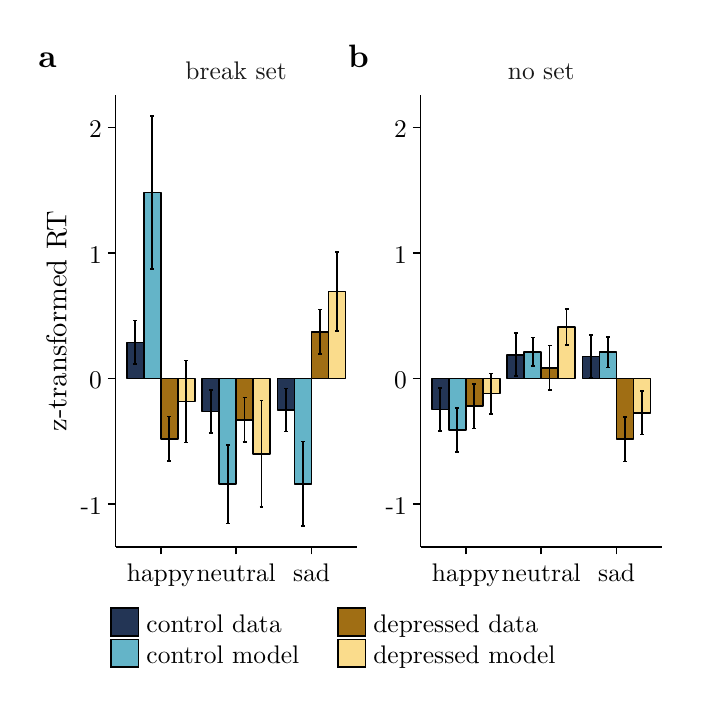
\begin{tikzpicture}[x=1pt,y=1pt]
\definecolor{fillColor}{RGB}{255,255,255}
\path[use as bounding box,fill=fillColor,fill opacity=0.00] (0,0) rectangle (234.88,234.88);
\begin{scope}
\path[clip] (  0.00, 28.91) rectangle (234.64,234.88);
\definecolor{drawColor}{RGB}{255,255,255}
\definecolor{fillColor}{RGB}{255,255,255}

\path[draw=drawColor,line width= 0.6pt,line join=round,line cap=round,fill=fillColor] (  0.00, 28.91) rectangle (234.64,234.88);
\end{scope}
\begin{scope}
\path[clip] ( 31.74, 47.29) rectangle (118.92,210.45);
\definecolor{fillColor}{RGB}{255,255,255}

\path[fill=fillColor] ( 31.74, 47.29) rectangle (118.92,210.45);
\definecolor{drawColor}{RGB}{0,0,0}
\definecolor{fillColor}{RGB}{250,220,140}

\path[draw=drawColor,line width= 0.6pt,line join=round,fill=fillColor] ( 54.22, 99.78) rectangle ( 60.35,108.16);
\definecolor{fillColor}{RGB}{160,110,20}

\path[draw=drawColor,line width= 0.6pt,line join=round,fill=fillColor] ( 48.09, 86.30) rectangle ( 54.22,108.16);
\definecolor{fillColor}{RGB}{100,180,200}

\path[draw=drawColor,line width= 0.6pt,line join=round,fill=fillColor] ( 41.96,108.16) rectangle ( 48.09,175.36);
\definecolor{fillColor}{RGB}{35,53,85}

\path[draw=drawColor,line width= 0.6pt,line join=round,fill=fillColor] ( 35.83,108.16) rectangle ( 41.96,121.17);
\definecolor{fillColor}{RGB}{250,220,140}

\path[draw=drawColor,line width= 0.6pt,line join=round,fill=fillColor] ( 81.46, 80.84) rectangle ( 87.59,108.16);
\definecolor{fillColor}{RGB}{160,110,20}

\path[draw=drawColor,line width= 0.6pt,line join=round,fill=fillColor] ( 75.33, 93.20) rectangle ( 81.46,108.16);
\definecolor{fillColor}{RGB}{100,180,200}

\path[draw=drawColor,line width= 0.6pt,line join=round,fill=fillColor] ( 69.20, 69.89) rectangle ( 75.33,108.16);
\definecolor{fillColor}{RGB}{35,53,85}

\path[draw=drawColor,line width= 0.6pt,line join=round,fill=fillColor] ( 63.07, 96.23) rectangle ( 69.20,108.16);
\definecolor{fillColor}{RGB}{250,220,140}

\path[draw=drawColor,line width= 0.6pt,line join=round,fill=fillColor] (108.71,108.16) rectangle (114.84,139.53);
\definecolor{fillColor}{RGB}{160,110,20}

\path[draw=drawColor,line width= 0.6pt,line join=round,fill=fillColor] (102.58,108.16) rectangle (108.71,124.98);
\definecolor{fillColor}{RGB}{100,180,200}

\path[draw=drawColor,line width= 0.6pt,line join=round,fill=fillColor] ( 96.45, 70.02) rectangle (102.58,108.16);
\definecolor{fillColor}{RGB}{35,53,85}

\path[draw=drawColor,line width= 0.6pt,line join=round,fill=fillColor] ( 90.32, 96.75) rectangle ( 96.45,108.16);

\path[draw=drawColor,line width= 0.6pt,line join=round] ( 56.60,114.59) --
	( 57.96,114.59);

\path[draw=drawColor,line width= 0.6pt,line join=round] ( 57.28,114.59) --
	( 57.28, 84.97);

\path[draw=drawColor,line width= 0.6pt,line join=round] ( 56.60, 84.97) --
	( 57.96, 84.97);

\path[draw=drawColor,line width= 0.6pt,line join=round] ( 50.47, 94.35) --
	( 51.83, 94.35);

\path[draw=drawColor,line width= 0.6pt,line join=round] ( 51.15, 94.35) --
	( 51.15, 78.26);

\path[draw=drawColor,line width= 0.6pt,line join=round] ( 50.47, 78.26) --
	( 51.83, 78.26);

\path[draw=drawColor,line width= 0.6pt,line join=round] ( 44.34,203.03) --
	( 45.70,203.03);

\path[draw=drawColor,line width= 0.6pt,line join=round] ( 45.02,203.03) --
	( 45.02,147.68);

\path[draw=drawColor,line width= 0.6pt,line join=round] ( 44.34,147.68) --
	( 45.70,147.68);

\path[draw=drawColor,line width= 0.6pt,line join=round] ( 38.21,129.12) --
	( 39.57,129.12);

\path[draw=drawColor,line width= 0.6pt,line join=round] ( 38.89,129.12) --
	( 38.89,113.23);

\path[draw=drawColor,line width= 0.6pt,line join=round] ( 38.21,113.23) --
	( 39.57,113.23);

\path[draw=drawColor,line width= 0.6pt,line join=round] ( 83.84,100.10) --
	( 85.21,100.10);

\path[draw=drawColor,line width= 0.6pt,line join=round] ( 84.53,100.10) --
	( 84.53, 61.58);

\path[draw=drawColor,line width= 0.6pt,line join=round] ( 83.84, 61.58) --
	( 85.21, 61.58);

\path[draw=drawColor,line width= 0.6pt,line join=round] ( 77.71,101.22) --
	( 79.08,101.22);

\path[draw=drawColor,line width= 0.6pt,line join=round] ( 78.40,101.22) --
	( 78.40, 85.17);

\path[draw=drawColor,line width= 0.6pt,line join=round] ( 77.71, 85.17) --
	( 79.08, 85.17);

\path[draw=drawColor,line width= 0.6pt,line join=round] ( 71.58, 84.03) --
	( 72.95, 84.03);

\path[draw=drawColor,line width= 0.6pt,line join=round] ( 72.27, 84.03) --
	( 72.27, 55.74);

\path[draw=drawColor,line width= 0.6pt,line join=round] ( 71.58, 55.74) --
	( 72.95, 55.74);

\path[draw=drawColor,line width= 0.6pt,line join=round] ( 65.45,103.97) --
	( 66.82,103.97);

\path[draw=drawColor,line width= 0.6pt,line join=round] ( 66.14,103.97) --
	( 66.14, 88.49);

\path[draw=drawColor,line width= 0.6pt,line join=round] ( 65.45, 88.49) --
	( 66.82, 88.49);

\path[draw=drawColor,line width= 0.6pt,line join=round] (111.09,153.71) --
	(112.45,153.71);

\path[draw=drawColor,line width= 0.6pt,line join=round] (111.77,153.71) --
	(111.77,125.34);

\path[draw=drawColor,line width= 0.6pt,line join=round] (111.09,125.34) --
	(112.45,125.34);

\path[draw=drawColor,line width= 0.6pt,line join=round] (104.96,133.03) --
	(106.32,133.03);

\path[draw=drawColor,line width= 0.6pt,line join=round] (105.64,133.03) --
	(105.64,116.93);

\path[draw=drawColor,line width= 0.6pt,line join=round] (104.96,116.93) --
	(106.32,116.93);

\path[draw=drawColor,line width= 0.6pt,line join=round] ( 98.83, 85.35) --
	(100.19, 85.35);

\path[draw=drawColor,line width= 0.6pt,line join=round] ( 99.51, 85.35) --
	( 99.51, 54.70);

\path[draw=drawColor,line width= 0.6pt,line join=round] ( 98.83, 54.70) --
	(100.19, 54.70);

\path[draw=drawColor,line width= 0.6pt,line join=round] ( 92.70,104.49) --
	( 94.06,104.49);

\path[draw=drawColor,line width= 0.6pt,line join=round] ( 93.38,104.49) --
	( 93.38, 89.01);

\path[draw=drawColor,line width= 0.6pt,line join=round] ( 92.70, 89.01) --
	( 94.06, 89.01);
\end{scope}
\begin{scope}
\path[clip] (141.96, 47.29) rectangle (229.14,210.45);
\definecolor{fillColor}{RGB}{255,255,255}

\path[fill=fillColor] (141.96, 47.29) rectangle (229.14,210.45);
\definecolor{drawColor}{RGB}{0,0,0}
\definecolor{fillColor}{RGB}{250,220,140}

\path[draw=drawColor,line width= 0.6pt,line join=round,fill=fillColor] (164.44,102.66) rectangle (170.57,108.16);
\definecolor{fillColor}{RGB}{160,110,20}

\path[draw=drawColor,line width= 0.6pt,line join=round,fill=fillColor] (158.31, 98.08) rectangle (164.44,108.16);
\definecolor{fillColor}{RGB}{100,180,200}

\path[draw=drawColor,line width= 0.6pt,line join=round,fill=fillColor] (152.18, 89.49) rectangle (158.31,108.16);
\definecolor{fillColor}{RGB}{35,53,85}

\path[draw=drawColor,line width= 0.6pt,line join=round,fill=fillColor] (146.05, 96.90) rectangle (152.18,108.16);
\definecolor{fillColor}{RGB}{250,220,140}

\path[draw=drawColor,line width= 0.6pt,line join=round,fill=fillColor] (191.68,108.16) rectangle (197.81,126.81);
\definecolor{fillColor}{RGB}{160,110,20}

\path[draw=drawColor,line width= 0.6pt,line join=round,fill=fillColor] (185.55,108.16) rectangle (191.68,111.97);
\definecolor{fillColor}{RGB}{100,180,200}

\path[draw=drawColor,line width= 0.6pt,line join=round,fill=fillColor] (179.42,108.16) rectangle (185.55,117.74);
\definecolor{fillColor}{RGB}{35,53,85}

\path[draw=drawColor,line width= 0.6pt,line join=round,fill=fillColor] (173.29,108.16) rectangle (179.42,116.70);
\definecolor{fillColor}{RGB}{250,220,140}

\path[draw=drawColor,line width= 0.6pt,line join=round,fill=fillColor] (218.93, 95.76) rectangle (225.06,108.16);
\definecolor{fillColor}{RGB}{160,110,20}

\path[draw=drawColor,line width= 0.6pt,line join=round,fill=fillColor] (212.80, 86.15) rectangle (218.93,108.16);
\definecolor{fillColor}{RGB}{100,180,200}

\path[draw=drawColor,line width= 0.6pt,line join=round,fill=fillColor] (206.67,108.16) rectangle (212.80,117.58);
\definecolor{fillColor}{RGB}{35,53,85}

\path[draw=drawColor,line width= 0.6pt,line join=round,fill=fillColor] (200.54,108.16) rectangle (206.67,116.03);

\path[draw=drawColor,line width= 0.6pt,line join=round] (166.82,109.93) --
	(168.18,109.93);

\path[draw=drawColor,line width= 0.6pt,line join=round] (167.50,109.93) --
	(167.50, 95.39);

\path[draw=drawColor,line width= 0.6pt,line join=round] (166.82, 95.39) --
	(168.18, 95.39);

\path[draw=drawColor,line width= 0.6pt,line join=round] (160.69,106.11) --
	(162.05,106.11);

\path[draw=drawColor,line width= 0.6pt,line join=round] (161.37,106.11) --
	(161.37, 90.06);

\path[draw=drawColor,line width= 0.6pt,line join=round] (160.69, 90.06) --
	(162.05, 90.06);

\path[draw=drawColor,line width= 0.6pt,line join=round] (154.56, 97.38) --
	(155.92, 97.38);

\path[draw=drawColor,line width= 0.6pt,line join=round] (155.24, 97.38) --
	(155.24, 81.61);

\path[draw=drawColor,line width= 0.6pt,line join=round] (154.56, 81.61) --
	(155.92, 81.61);

\path[draw=drawColor,line width= 0.6pt,line join=round] (148.43,104.66) --
	(149.79,104.66);

\path[draw=drawColor,line width= 0.6pt,line join=round] (149.11,104.66) --
	(149.11, 89.13);

\path[draw=drawColor,line width= 0.6pt,line join=round] (148.43, 89.13) --
	(149.79, 89.13);

\path[draw=drawColor,line width= 0.6pt,line join=round] (194.07,133.33) --
	(195.43,133.33);

\path[draw=drawColor,line width= 0.6pt,line join=round] (194.75,133.33) --
	(194.75,120.30);

\path[draw=drawColor,line width= 0.6pt,line join=round] (194.07,120.30) --
	(195.43,120.30);

\path[draw=drawColor,line width= 0.6pt,line join=round] (187.93,120.02) --
	(189.30,120.02);

\path[draw=drawColor,line width= 0.6pt,line join=round] (188.62,120.02) --
	(188.62,103.92);

\path[draw=drawColor,line width= 0.6pt,line join=round] (187.93,103.92) --
	(189.30,103.92);

\path[draw=drawColor,line width= 0.6pt,line join=round] (181.80,122.91) --
	(183.17,122.91);

\path[draw=drawColor,line width= 0.6pt,line join=round] (182.49,122.91) --
	(182.49,112.58);

\path[draw=drawColor,line width= 0.6pt,line join=round] (181.80,112.58) --
	(183.17,112.58);

\path[draw=drawColor,line width= 0.6pt,line join=round] (175.67,124.44) --
	(177.04,124.44);

\path[draw=drawColor,line width= 0.6pt,line join=round] (176.36,124.44) --
	(176.36,108.96);

\path[draw=drawColor,line width= 0.6pt,line join=round] (175.67,108.96) --
	(177.04,108.96);

\path[draw=drawColor,line width= 0.6pt,line join=round] (221.31,103.62) --
	(222.67,103.62);

\path[draw=drawColor,line width= 0.6pt,line join=round] (221.99,103.62) --
	(221.99, 87.90);

\path[draw=drawColor,line width= 0.6pt,line join=round] (221.31, 87.90) --
	(222.67, 87.90);

\path[draw=drawColor,line width= 0.6pt,line join=round] (215.18, 94.17) --
	(216.54, 94.17);

\path[draw=drawColor,line width= 0.6pt,line join=round] (215.86, 94.17) --
	(215.86, 78.12);

\path[draw=drawColor,line width= 0.6pt,line join=round] (215.18, 78.12) --
	(216.54, 78.12);

\path[draw=drawColor,line width= 0.6pt,line join=round] (209.05,123.04) --
	(210.41,123.04);

\path[draw=drawColor,line width= 0.6pt,line join=round] (209.73,123.04) --
	(209.73,112.13);

\path[draw=drawColor,line width= 0.6pt,line join=round] (209.05,112.13) --
	(210.41,112.13);

\path[draw=drawColor,line width= 0.6pt,line join=round] (202.92,123.77) --
	(204.28,123.77);

\path[draw=drawColor,line width= 0.6pt,line join=round] (203.60,123.77) --
	(203.60,108.29);

\path[draw=drawColor,line width= 0.6pt,line join=round] (202.92,108.29) --
	(204.28,108.29);
\end{scope}
\begin{scope}
\path[clip] ( 31.74,210.45) rectangle (118.92,229.38);
\definecolor{drawColor}{RGB}{255,255,255}
\definecolor{fillColor}{RGB}{255,255,255}

\path[draw=drawColor,line width= 1.1pt,line join=round,line cap=round,fill=fillColor] ( 31.74,210.45) rectangle (118.92,229.38);
\definecolor{drawColor}{gray}{0.10}

\node[text=drawColor,anchor=base,inner sep=0pt, outer sep=0pt, scale=  0.92] at ( 75.33,216.13) {break set};
\end{scope}
\begin{scope}
\path[clip] (141.96,210.45) rectangle (229.14,229.38);
\definecolor{drawColor}{RGB}{255,255,255}
\definecolor{fillColor}{RGB}{255,255,255}

\path[draw=drawColor,line width= 1.1pt,line join=round,line cap=round,fill=fillColor] (141.96,210.45) rectangle (229.14,229.38);
\definecolor{drawColor}{gray}{0.10}

\node[text=drawColor,anchor=base,inner sep=0pt, outer sep=0pt, scale=  0.92] at (185.55,216.13) {no set};
\end{scope}
\begin{scope}
\path[clip] (  0.00,  0.00) rectangle (234.88,234.88);
\definecolor{drawColor}{RGB}{0,0,0}

\path[draw=drawColor,line width= 0.6pt,line join=round] ( 31.74, 47.29) --
	(118.92, 47.29);
\end{scope}
\begin{scope}
\path[clip] (  0.00,  0.00) rectangle (234.88,234.88);
\definecolor{drawColor}{RGB}{0,0,0}

\path[draw=drawColor,line width= 0.6pt,line join=round] ( 48.09, 44.54) --
	( 48.09, 47.29);

\path[draw=drawColor,line width= 0.6pt,line join=round] ( 75.33, 44.54) --
	( 75.33, 47.29);

\path[draw=drawColor,line width= 0.6pt,line join=round] (102.58, 44.54) --
	(102.58, 47.29);
\end{scope}
\begin{scope}
\path[clip] (  0.00,  0.00) rectangle (234.88,234.88);
\definecolor{drawColor}{RGB}{0,0,0}

\node[text=drawColor,anchor=base,inner sep=0pt, outer sep=0pt, scale=  0.92] at ( 48.09, 34.76) {happy};

\node[text=drawColor,anchor=base,inner sep=0pt, outer sep=0pt, scale=  0.92] at ( 75.33, 34.76) {neutral};

\node[text=drawColor,anchor=base,inner sep=0pt, outer sep=0pt, scale=  0.92] at (102.58, 34.76) {sad};
\end{scope}
\begin{scope}
\path[clip] (  0.00,  0.00) rectangle (234.88,234.88);
\definecolor{drawColor}{RGB}{0,0,0}

\path[draw=drawColor,line width= 0.6pt,line join=round] (141.96, 47.29) --
	(229.14, 47.29);
\end{scope}
\begin{scope}
\path[clip] (  0.00,  0.00) rectangle (234.88,234.88);
\definecolor{drawColor}{RGB}{0,0,0}

\path[draw=drawColor,line width= 0.6pt,line join=round] (158.31, 44.54) --
	(158.31, 47.29);

\path[draw=drawColor,line width= 0.6pt,line join=round] (185.55, 44.54) --
	(185.55, 47.29);

\path[draw=drawColor,line width= 0.6pt,line join=round] (212.80, 44.54) --
	(212.80, 47.29);
\end{scope}
\begin{scope}
\path[clip] (  0.00,  0.00) rectangle (234.88,234.88);
\definecolor{drawColor}{RGB}{0,0,0}

\node[text=drawColor,anchor=base,inner sep=0pt, outer sep=0pt, scale=  0.92] at (158.31, 34.76) {happy};

\node[text=drawColor,anchor=base,inner sep=0pt, outer sep=0pt, scale=  0.92] at (185.55, 34.76) {neutral};

\node[text=drawColor,anchor=base,inner sep=0pt, outer sep=0pt, scale=  0.92] at (212.80, 34.76) {sad};
\end{scope}
\begin{scope}
\path[clip] (  0.00,  0.00) rectangle (234.88,234.88);
\definecolor{drawColor}{RGB}{0,0,0}

\path[draw=drawColor,line width= 0.6pt,line join=round] ( 31.74, 47.29) --
	( 31.74,210.45);
\end{scope}
\begin{scope}
\path[clip] (  0.00,  0.00) rectangle (234.88,234.88);
\definecolor{drawColor}{RGB}{0,0,0}

\node[text=drawColor,anchor=base east,inner sep=0pt, outer sep=0pt, scale=  0.92] at ( 26.79, 59.04) {-1};

\node[text=drawColor,anchor=base east,inner sep=0pt, outer sep=0pt, scale=  0.92] at ( 26.79,104.37) {0};

\node[text=drawColor,anchor=base east,inner sep=0pt, outer sep=0pt, scale=  0.92] at ( 26.79,149.71) {1};

\node[text=drawColor,anchor=base east,inner sep=0pt, outer sep=0pt, scale=  0.92] at ( 26.79,195.04) {2};
\end{scope}
\begin{scope}
\path[clip] (  0.00,  0.00) rectangle (234.88,234.88);
\definecolor{drawColor}{RGB}{0,0,0}

\path[draw=drawColor,line width= 0.6pt,line join=round] ( 28.99, 62.83) --
	( 31.74, 62.83);

\path[draw=drawColor,line width= 0.6pt,line join=round] ( 28.99,108.16) --
	( 31.74,108.16);

\path[draw=drawColor,line width= 0.6pt,line join=round] ( 28.99,153.50) --
	( 31.74,153.50);

\path[draw=drawColor,line width= 0.6pt,line join=round] ( 28.99,198.83) --
	( 31.74,198.83);
\end{scope}
\begin{scope}
\path[clip] (  0.00,  0.00) rectangle (234.88,234.88);
\definecolor{drawColor}{RGB}{0,0,0}

\path[draw=drawColor,line width= 0.6pt,line join=round] (141.96, 47.29) --
	(141.96,210.45);
\end{scope}
\begin{scope}
\path[clip] (  0.00,  0.00) rectangle (234.88,234.88);
\definecolor{drawColor}{RGB}{0,0,0}

\node[text=drawColor,anchor=base east,inner sep=0pt, outer sep=0pt, scale=  0.92] at (137.01, 59.04) {-1};

\node[text=drawColor,anchor=base east,inner sep=0pt, outer sep=0pt, scale=  0.92] at (137.01,104.37) {0};

\node[text=drawColor,anchor=base east,inner sep=0pt, outer sep=0pt, scale=  0.92] at (137.01,149.71) {1};

\node[text=drawColor,anchor=base east,inner sep=0pt, outer sep=0pt, scale=  0.92] at (137.01,195.04) {2};
\end{scope}
\begin{scope}
\path[clip] (  0.00,  0.00) rectangle (234.88,234.88);
\definecolor{drawColor}{RGB}{0,0,0}

\path[draw=drawColor,line width= 0.6pt,line join=round] (139.21, 62.83) --
	(141.96, 62.83);

\path[draw=drawColor,line width= 0.6pt,line join=round] (139.21,108.16) --
	(141.96,108.16);

\path[draw=drawColor,line width= 0.6pt,line join=round] (139.21,153.50) --
	(141.96,153.50);

\path[draw=drawColor,line width= 0.6pt,line join=round] (139.21,198.83) --
	(141.96,198.83);
\end{scope}
\begin{scope}
\path[clip] (  0.00,  0.00) rectangle (234.88,234.88);
\definecolor{drawColor}{RGB}{0,0,0}

\node[text=drawColor,rotate= 90.00,anchor=base,inner sep=0pt, outer sep=0pt, scale=  1.03] at ( 14.02,128.87) {z-transformed RT};
\end{scope}
\begin{scope}
\path[clip] (  0.00,  0.00) rectangle (234.88,234.88);
\definecolor{drawColor}{RGB}{0,0,0}

\node[text=drawColor,anchor=base west,inner sep=0pt, outer sep=0pt, scale=  1.17] at (  3.83,220.38) {\bfseries a};

\node[text=drawColor,anchor=base west,inner sep=0pt, outer sep=0pt, scale=  1.17] at (115.83,220.38) {\bfseries b};
\end{scope}
\begin{scope}
\path[clip] (  0.00,  0.00) rectangle (234.88,234.88);
\definecolor{fillColor}{RGB}{255,255,255}

\path[fill=fillColor] ( 19.35, -2.62) rectangle (215.29, 31.53);
\end{scope}
\begin{scope}
\path[clip] (  0.00,  0.00) rectangle (234.88,234.88);
\definecolor{drawColor}{RGB}{0,0,0}
\definecolor{fillColor}{RGB}{35,53,85}

\path[draw=drawColor,line width= 0.6pt,line cap=round,fill=fillColor] ( 30.09, 15.17) rectangle ( 40.05, 25.12);
\end{scope}
\begin{scope}
\path[clip] (  0.00,  0.00) rectangle (234.88,234.88);
\definecolor{drawColor}{RGB}{0,0,0}
\definecolor{fillColor}{RGB}{100,180,200}

\path[draw=drawColor,line width= 0.6pt,line cap=round,fill=fillColor] ( 30.09,  3.78) rectangle ( 40.05, 13.74);
\end{scope}
\begin{scope}
\path[clip] (  0.00,  0.00) rectangle (234.88,234.88);
\definecolor{drawColor}{RGB}{0,0,0}
\definecolor{fillColor}{RGB}{160,110,20}

\path[draw=drawColor,line width= 0.6pt,line cap=round,fill=fillColor] (112.08, 15.17) rectangle (122.03, 25.12);
\end{scope}
\begin{scope}
\path[clip] (  0.00,  0.00) rectangle (234.88,234.88);
\definecolor{drawColor}{RGB}{0,0,0}
\definecolor{fillColor}{RGB}{250,220,140}

\path[draw=drawColor,line width= 0.6pt,line cap=round,fill=fillColor] (112.08,  3.78) rectangle (122.03, 13.74);
\end{scope}
\begin{scope}
\path[clip] (  0.00,  0.00) rectangle (234.88,234.88);
\definecolor{drawColor}{RGB}{0,0,0}

\node[text=drawColor,anchor=base west,inner sep=0pt, outer sep=0pt, scale=  0.92] at ( 42.93, 16.36) {control data};
\end{scope}
\begin{scope}
\path[clip] (  0.00,  0.00) rectangle (234.88,234.88);
\definecolor{drawColor}{RGB}{0,0,0}

\node[text=drawColor,anchor=base west,inner sep=0pt, outer sep=0pt, scale=  0.92] at ( 42.93,  4.98) {control model};
\end{scope}
\begin{scope}
\path[clip] (  0.00,  0.00) rectangle (234.88,234.88);
\definecolor{drawColor}{RGB}{0,0,0}

\node[text=drawColor,anchor=base west,inner sep=0pt, outer sep=0pt, scale=  0.92] at (124.91, 16.36) {depressed data};
\end{scope}
\begin{scope}
\path[clip] (  0.00,  0.00) rectangle (234.88,234.88);
\definecolor{drawColor}{RGB}{0,0,0}

\node[text=drawColor,anchor=base west,inner sep=0pt, outer sep=0pt, scale=  0.92] at (124.91,  4.98) {depressed model};
\end{scope}
\end{tikzpicture}
